\documentclass[main]{subfiles} 
\graphicspath{{img/}}


\begin{document}

\section{Results}
The implementation of all the programs contained in the project result in obtaining the data from the web scrapper,
then transforming it to build the \ac{gui}.
This will help the user to get information on the lausanne housing market, see price listings, historical listings and navigate easily between available properties.

\subsection{Dataset}
The dataset we used for the building the \ac{gui} is reduced compared to all the data we initially have access to. 
We chose to keep this reduced version of the dataset, to keep the \ac{gui} easy to use and read for the user. 
Figure \ref{fig:propcodes} and \ref{fig:propdetails} show the the first few rows of the two cvs files: \pkg[property\_codes.csv] and \pkg[property\_details.csv] returned from the webscrapping.
Figure \ref{fig:dataxlsx} shows the data we used to feed the \ac{gui}.
Figure \ref{fig:graph1} shows the data we used for the average price by zip code graph.
Figure \ref{fig:graph2} shows the data we used for the average price by number of rooms graph.

\begin{figure}[htbp]
    \centerline{
        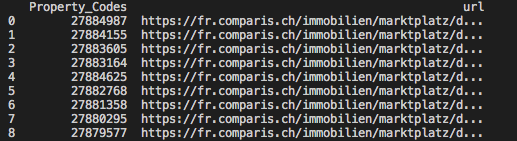
\includegraphics[width = 92mm]{prog_13.png}}
    \caption{First rows of \pkg[property\_codes.csv]}
    \label{fig:propcodes}
\end{figure}

\begin{figure}[htbp]
    \centerline{
        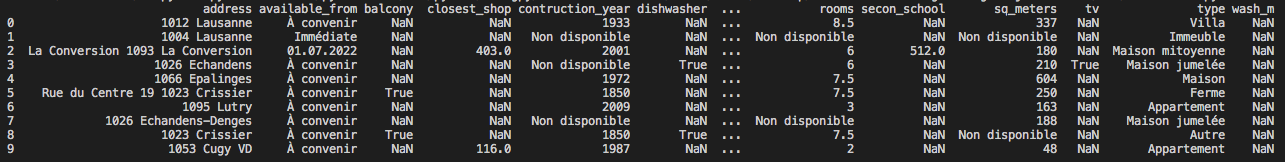
\includegraphics[width = 110mm]{prog_14.png}}
    \caption{First rows of \pkg[property\_details.csv]}
    \label{fig:propdetails}
\end{figure}

\begin{figure}[htbp]
    \centerline{
        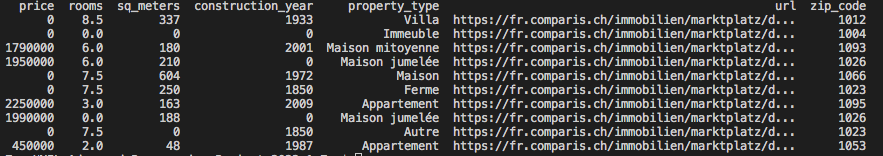
\includegraphics[width = 92mm]{prog_15.png}}
    \caption{First rows of \pkg[data.xlsx]}
    \label{fig:dataxlsx}
\end{figure}

\begin{figure}[htbp]
    \centerline{
        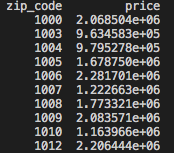
\includegraphics[width = 92mm]{prog_16.png}}
    \caption{First rows of data used for the average price by zip code graph}
    \label{fig:graph1}
\end{figure}

\begin{figure}[htbp]
    \centerline{
        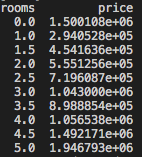
\includegraphics[width = 92mm]{prog_17.png}}
    \caption{First rows of data used for the average price by number of rooms graph}
    \label{fig:graph2}
\end{figure}



\subsection{\ac{gui}}
The \ac{gui} presents the scrapped data in an orderly manner.


\subsubsection{Main Window}
The main window contains the four available tabs namely, price range, Rooms, 
Zip Code and Graphs and the empty treeview. (see \ref{fig:Main_Window})

\begin{figure}[htbp]
    \centerline{
        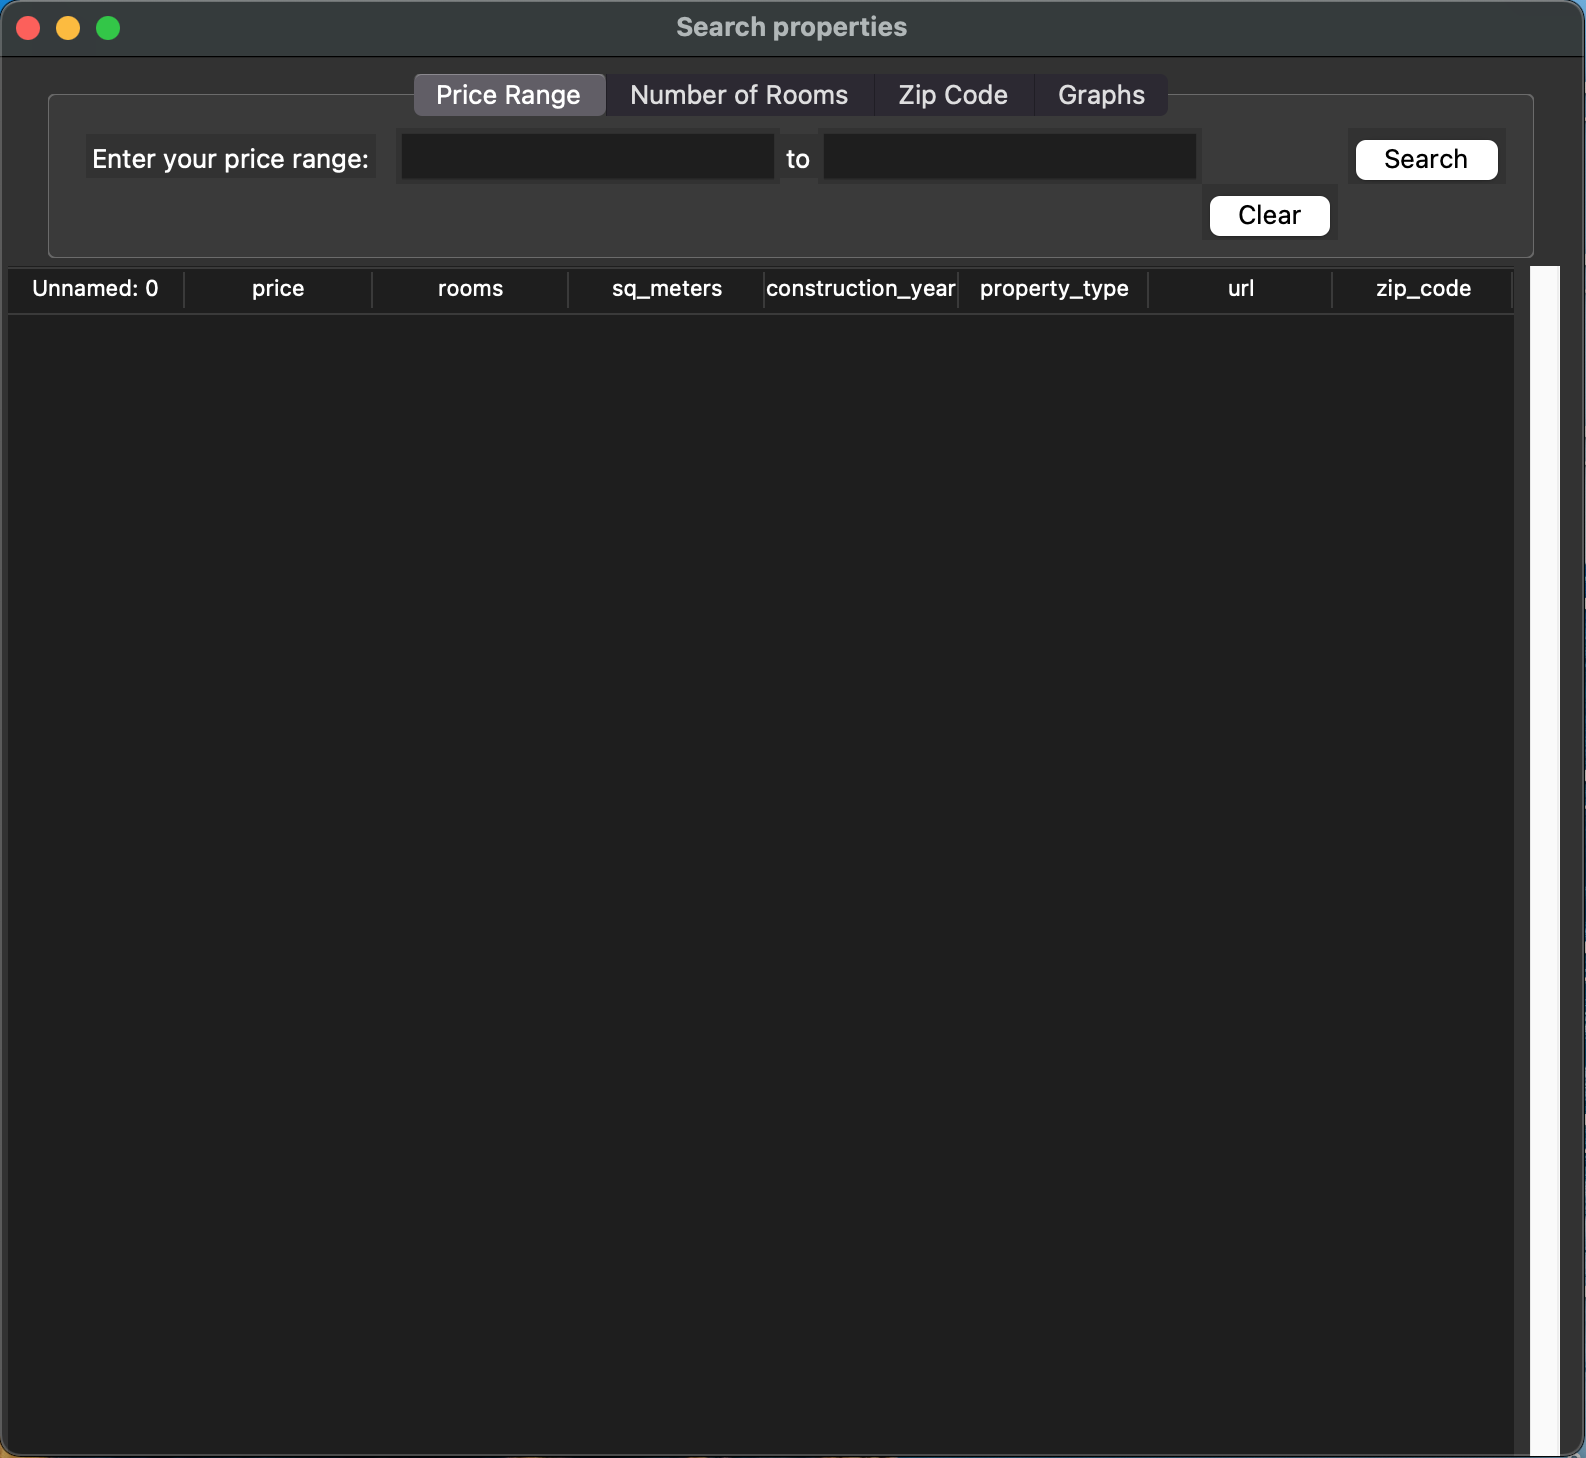
\includegraphics[width = 92mm]{prog_7.png}}
    \caption{View of the main window}
    \label{fig:Main_Window}
\end{figure}

\subsubsection{Frame 1}
The first frame allows the user to search within a specific price range. 
The user enters a minimum value and maximum value within each of the boxes and presses the search button. 
The treeview returns all the properties within the chosen price range. (see \ref{fig:frame1})
To restart the process, the user can either press the clear button or enter new values.

\begin{figure}[htbp]
    \centerline{
        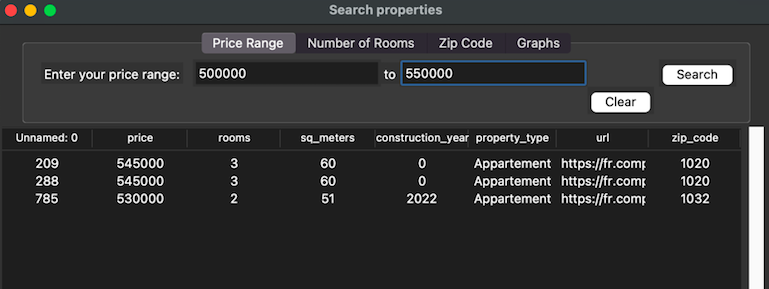
\includegraphics[width = 92mm]{prog_8.png}}
    \caption{View of the first frame}
    \label{fig:frame1}
\end{figure}

\subsubsection{Frame 2}
The second frame allows the user to search within a specific number of rooms. 
The user enters a minimum value and maximum value within each of the boxes and presses the search button. 
The treeview returns all the properties within the chosen number of rooms. (see \ref{fig:frame2})
To restart the process, the user can either press the clear button or enter new values.

\begin{figure}[htbp]
    \centerline{
        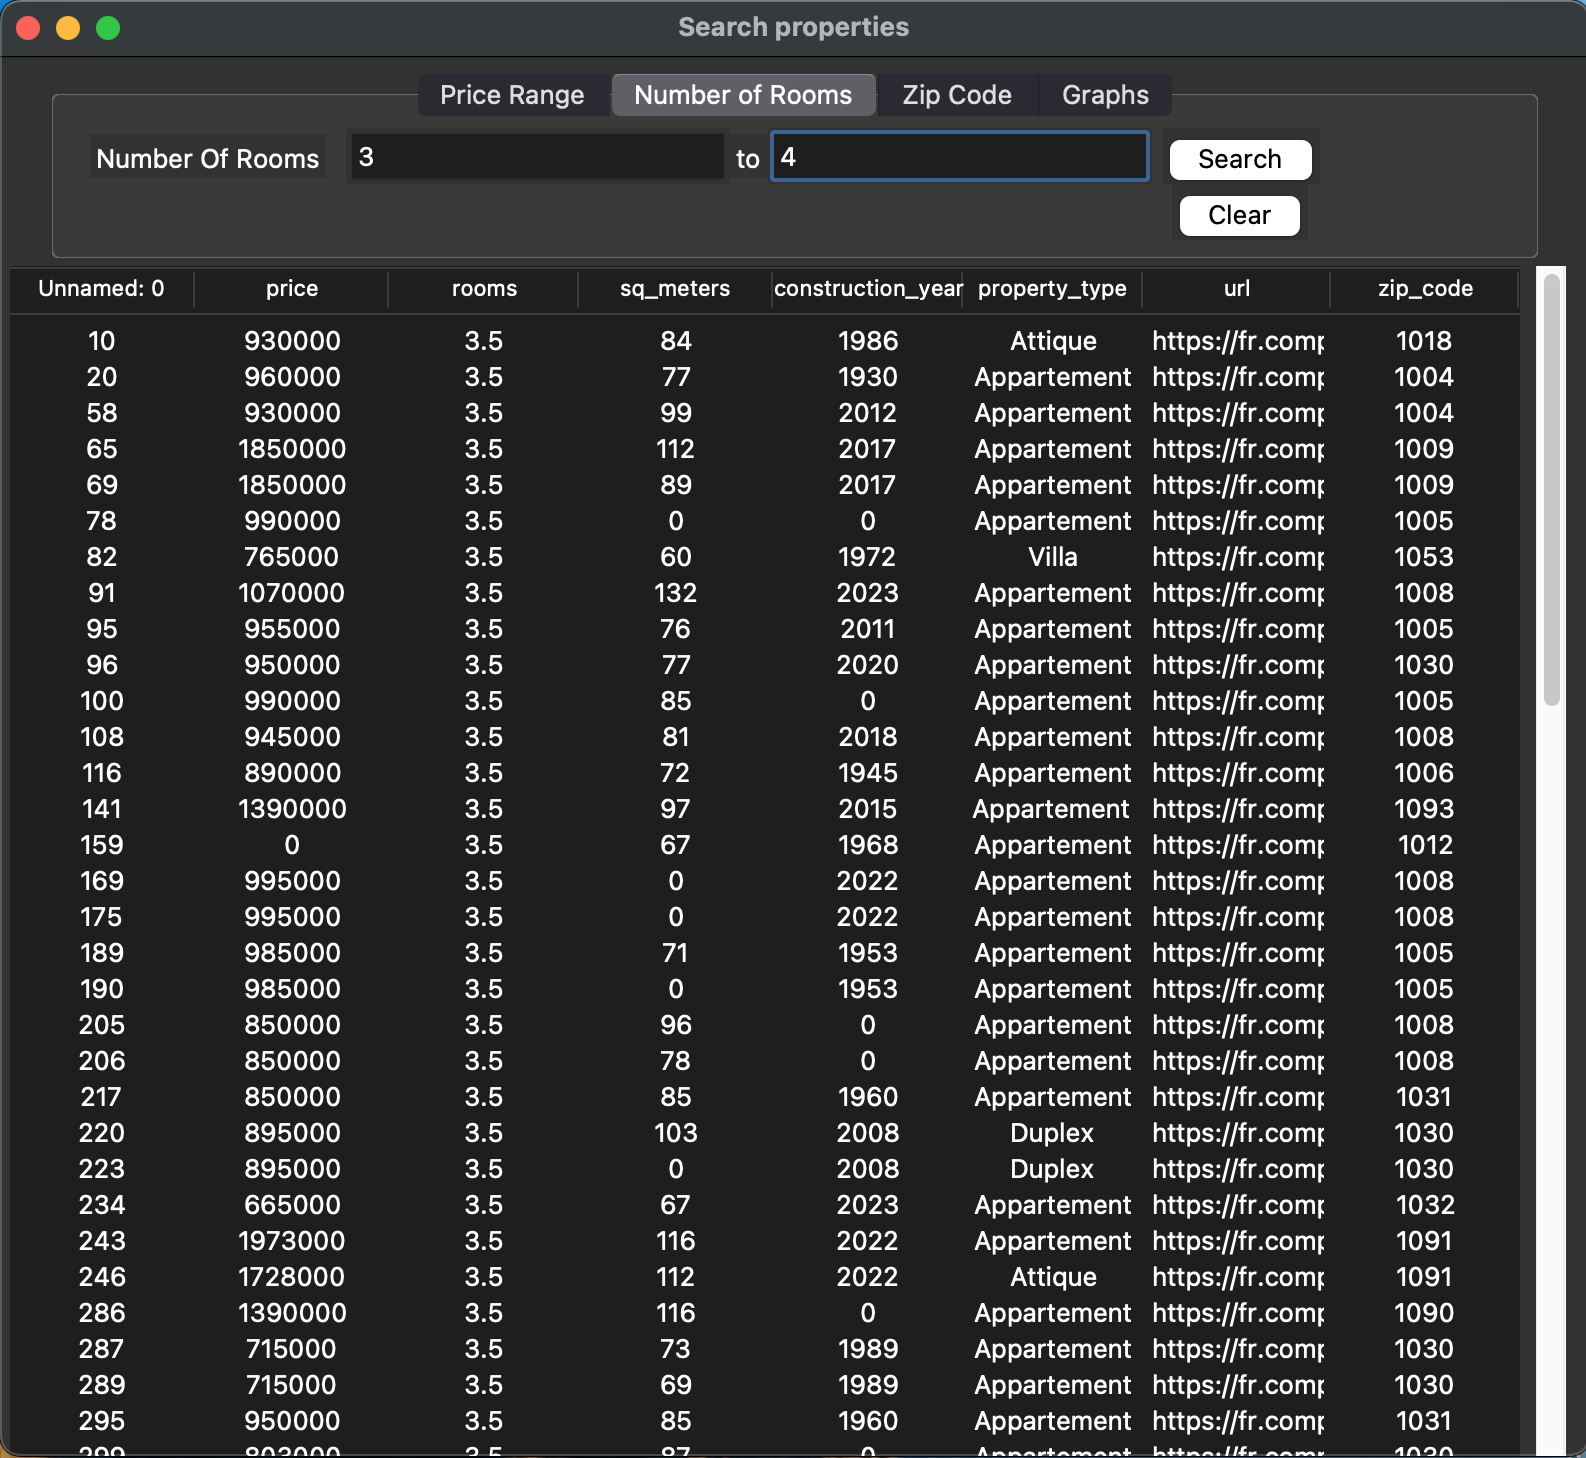
\includegraphics[width = 92mm]{prog_9.png}}
    \caption{View of the second frame}
    \label{fig:frame2}
\end{figure}

\subsubsection{Frame 3}
The third frame allows the user to search for properties in a specific zip code. 
The user enters the wished zip code in the box and presses the search button. 
The treeview returns all the properties within the chosen zip code.(see \ref{fig:frame3})
To restart the process, the user can either press the clear button or enter a new value.

\begin{figure}[htbp]
    \centerline{
        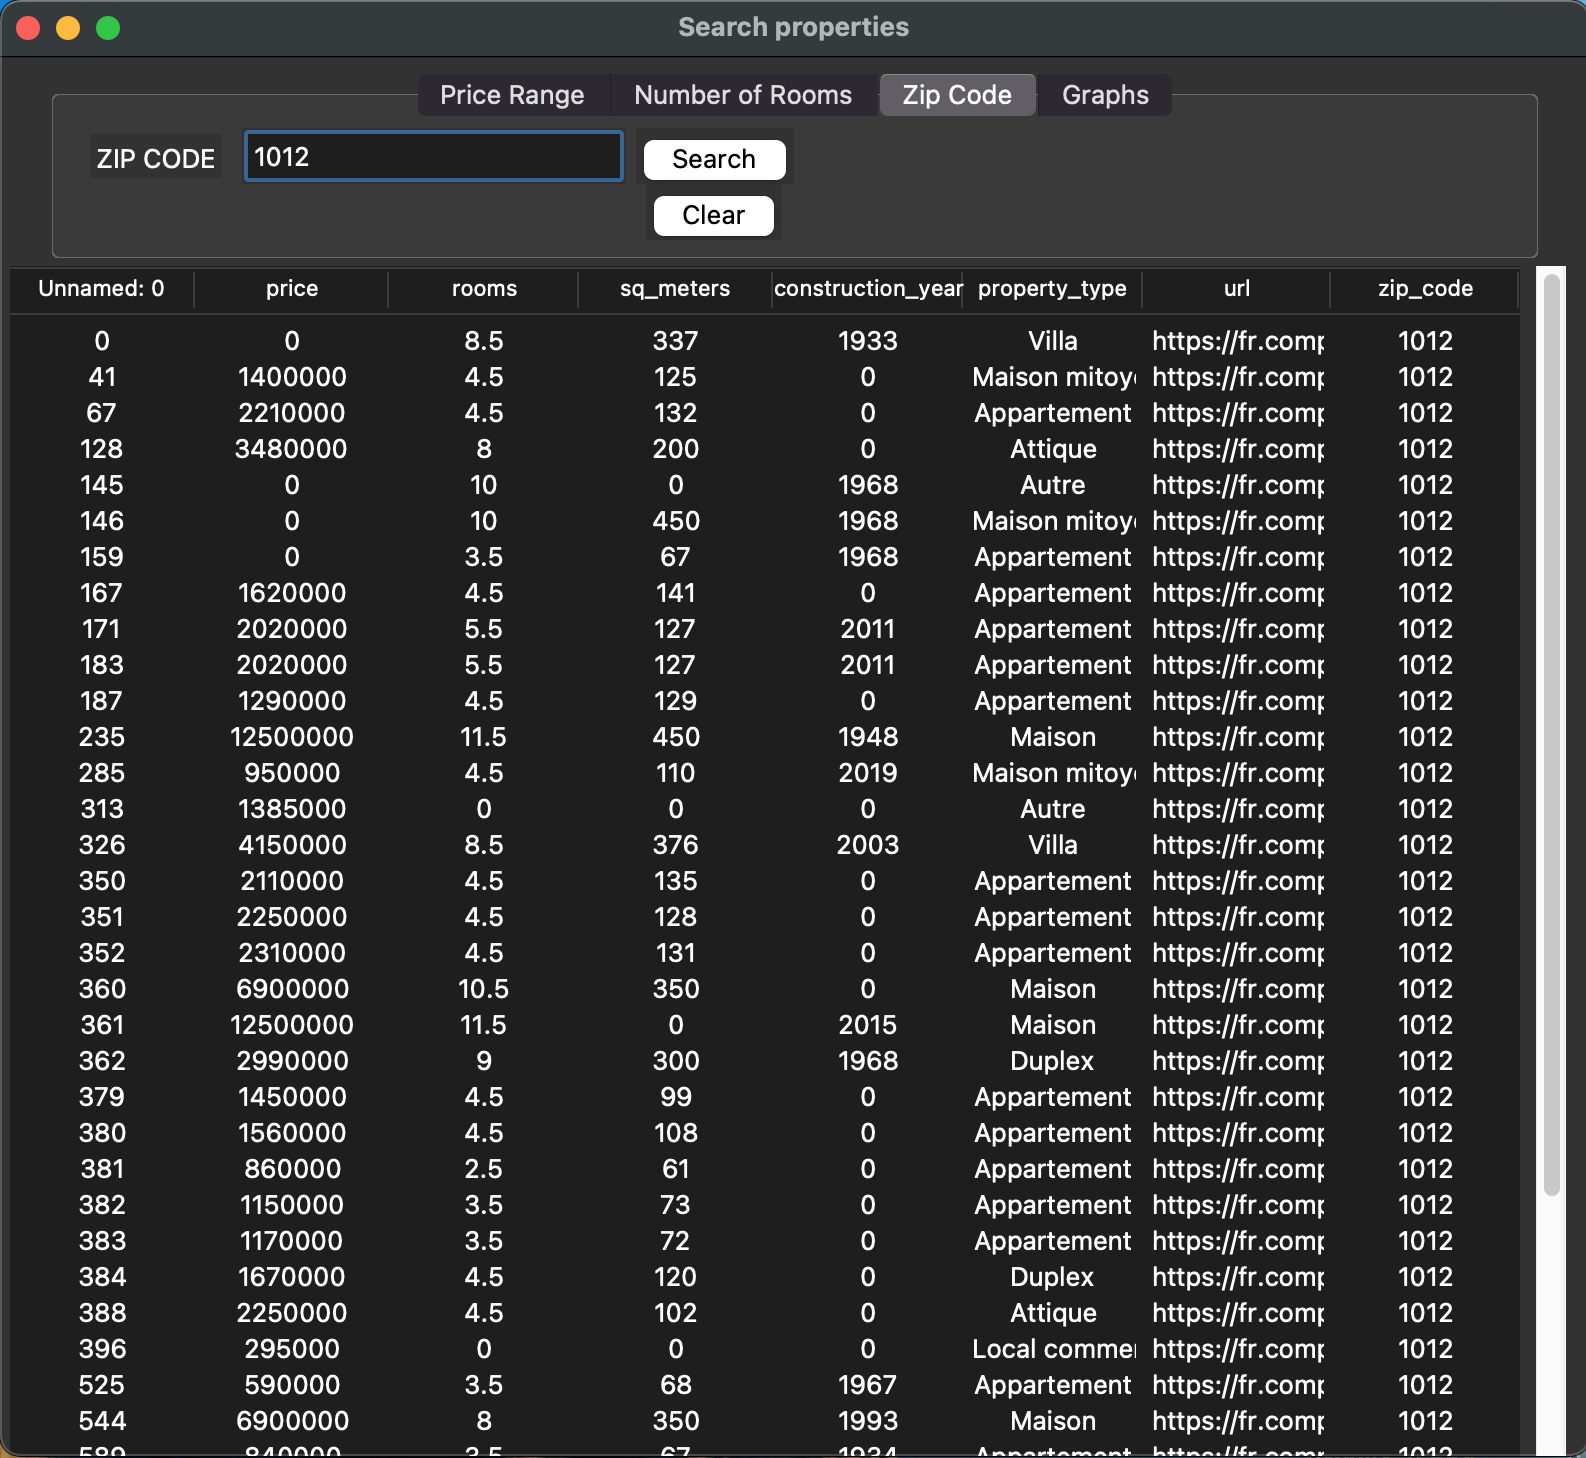
\includegraphics[width = 92mm]{prog_10.png}}
    \caption{View of the third frame}
    \label{fig:frame3}
\end{figure}

\subsubsection{Frame 4}
The fourth frame displays two buttons corresponding to two different bar graphs, 
namely the average price by zip code and the average price by number of rooms.
The user must simply press on the corresponding button and the graph is displayed. 
The figure \ref{fig:pricebyzip} displays the average price per zip code in millions of CHF. 
At the time when we run the program we can see that the zip code 1094 correspnding to Belmont sur Lausanne has the highest average price, namely of $3.7$ million CHF.
In general, the zip codes corresponding to the outskirts of Lausanne have a higher average price. 
This could be due to those areas being less built up, hence the properties there tend to be houses and villas rather than apartments. 
has a much higher price. 

\begin{figure}[htbp]
    \centerline{
        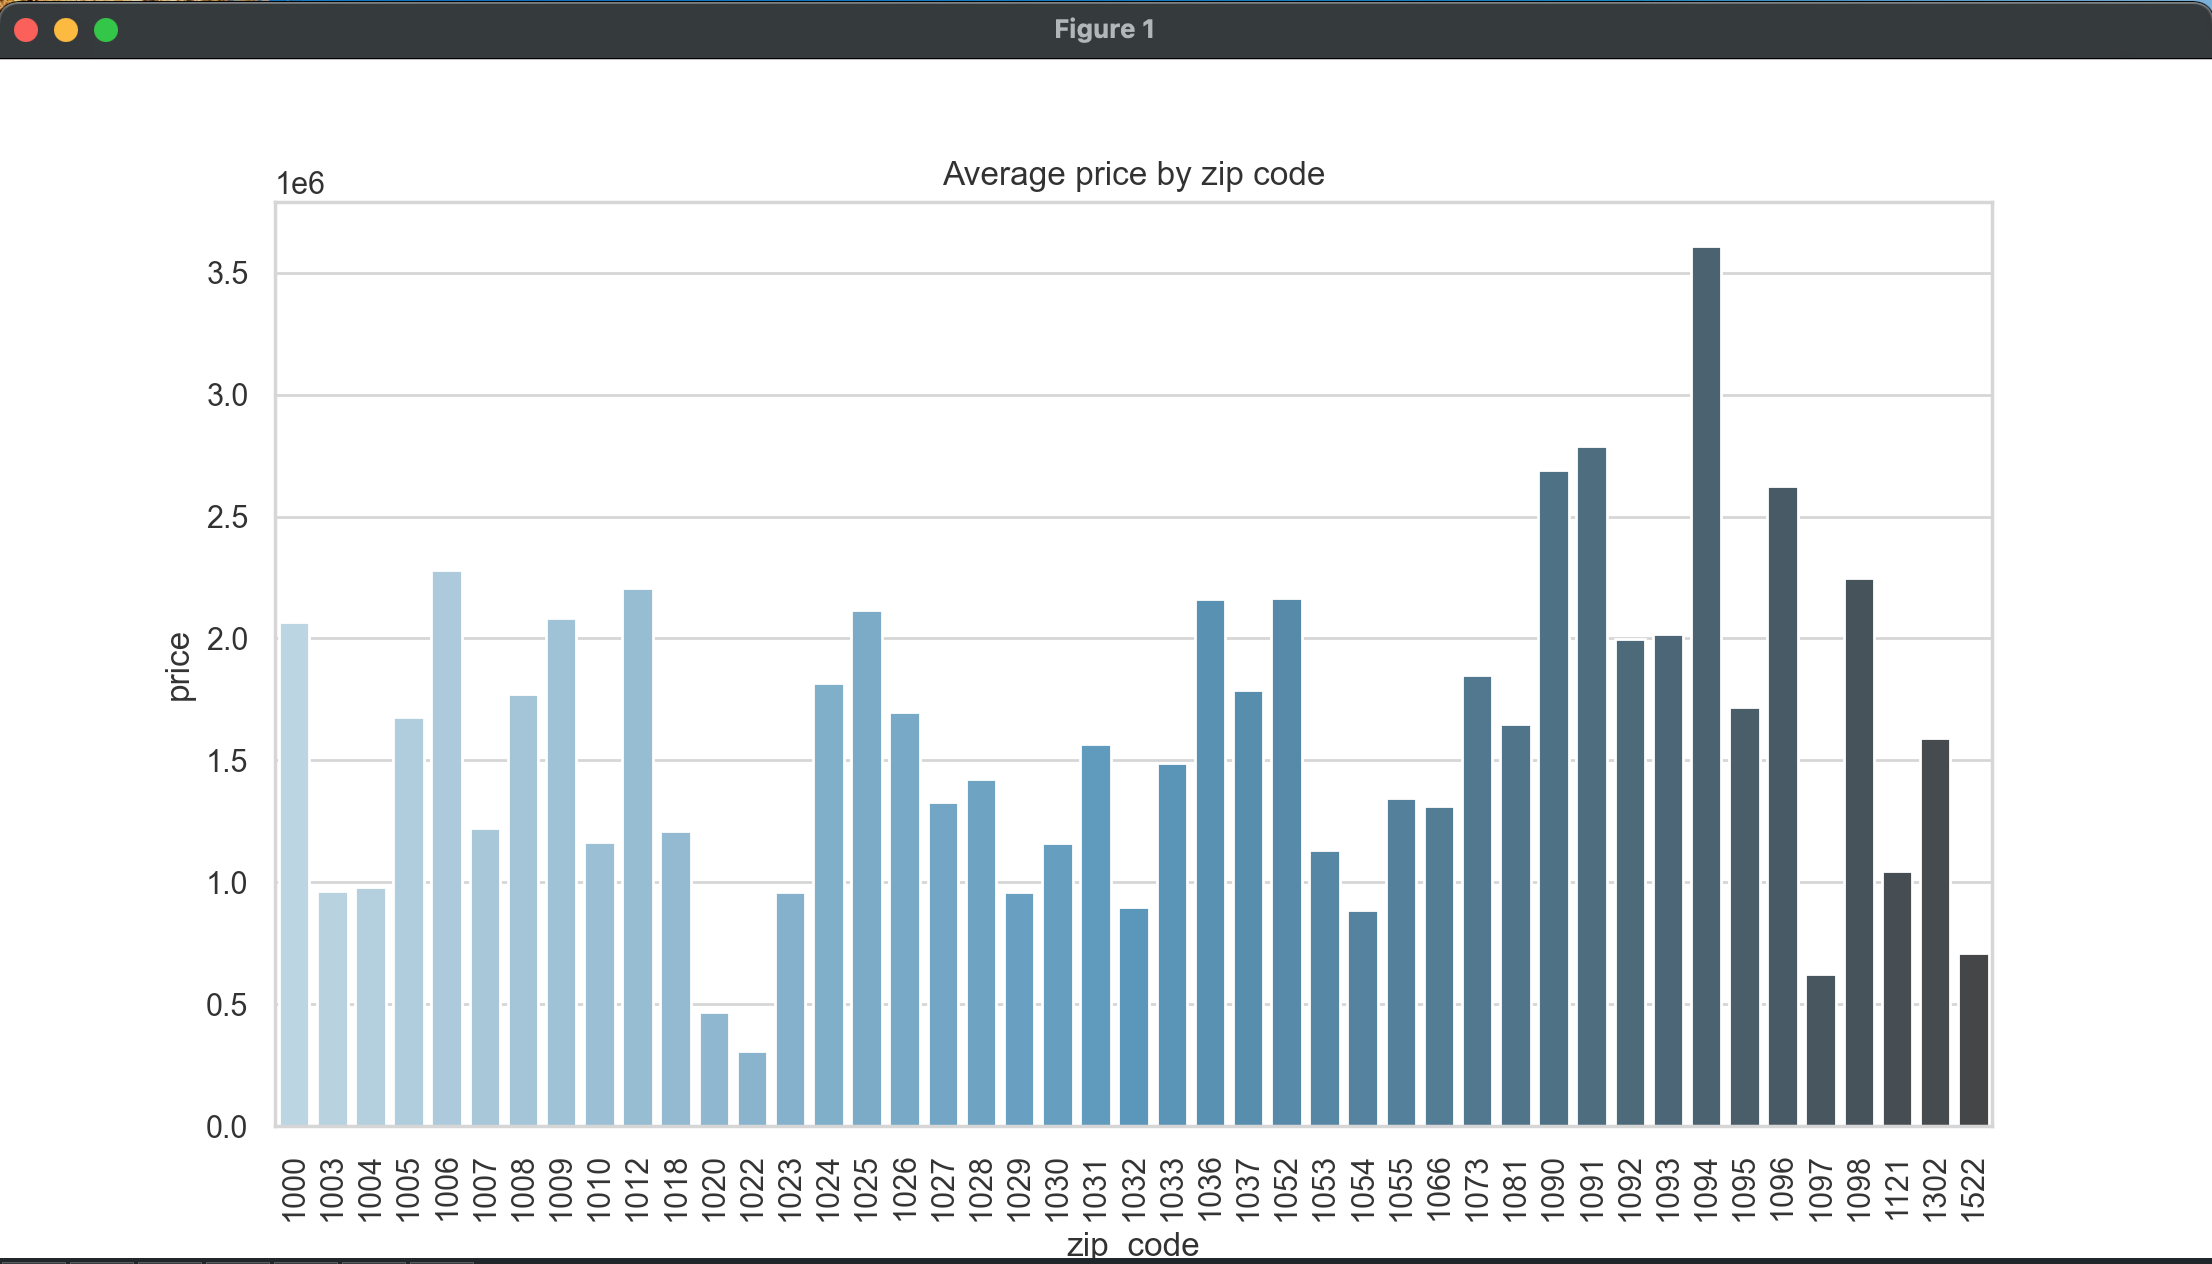
\includegraphics[width = 92mm]{prog_11.png}}
    \caption{Average price by zip code}
    \label{fig:pricebyzip}
\end{figure}


The figure \ref{fig:pricebyrooms} displays the average price per number of rooms by a base of 10 million CHF . 
At the time when we run the program we can see that the price per number of rooms does not grow exponentially as the number of rooms increases.
This could be due to the dataset containing many types of properties such as: commercial properties, apartments, houses and hotels, which messes with overall average. 
Moreover a lack of data can also explain the lack of exponential growth as the number of rooms increases. 

\begin{figure}[htbp]
    \centerline{
        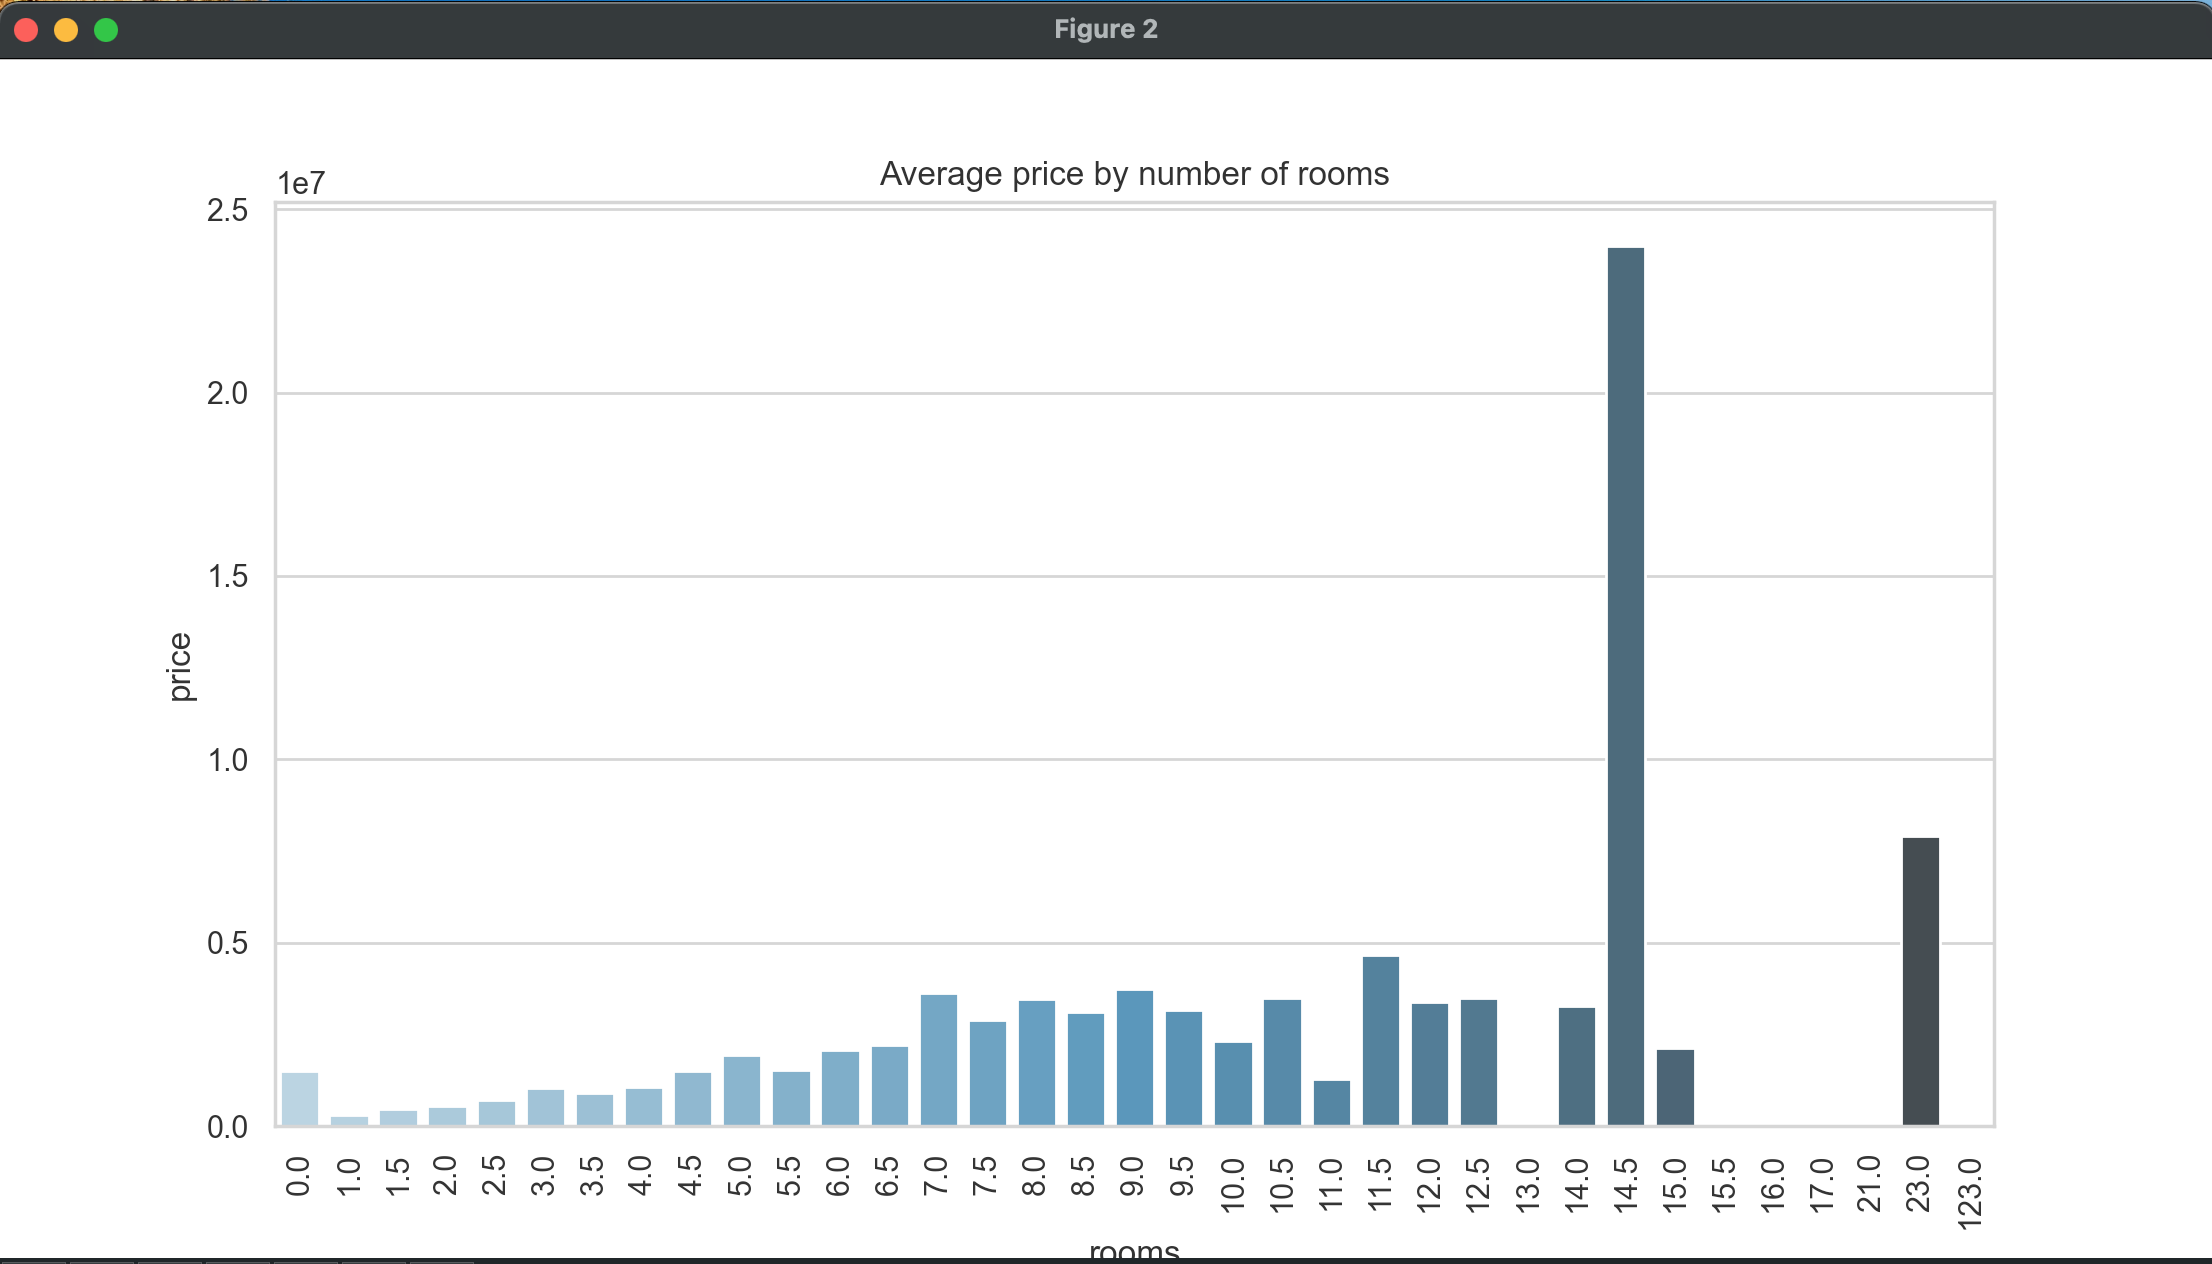
\includegraphics[width = 92mm]{prog_12.png}}
    \caption{Average price by zip code}
    \label{fig:pricebyrooms}
\end{figure}

\subsubsection{Heatmap}
Iniatially we wanted to display a heatmap of Lausanne based on the average price by zip code. 
This map is built with the help of the geopandas and folium packages. 
To build it we merge the MeanPriceZip file with the geolocations of the Lausanne's zip codes. Nonetheless, 
due to a merging and geolocation issue we were unable to display the map. 
\end{document}